\documentclass{note}
\usepackage{tikz}
\usepackage{diagbox}
\usetikzlibrary{graphs,positioning}
\tikzset{
    red/.style ={
        shape=circle,
        scale=1.5,
        draw=red,
        fill=red,
        text=white,
        minimum size=20pt
    },
    black/.style ={
        shape=circle,
        scale=1.5,
        draw=black,
        fill=black,
        text=white,
        minimum size=20pt
    }
}
\title{红黑树}
\author{宋星霖}
\date{\today}
\begin{document}
\maketitle
\section{结构讲解}
红黑树是一种平衡二叉树排序树,其有以下几种平衡条件:
\begin{enumerate}
    \item 每个节点非黑即红
    \item 根节点是黑色
    \item 叶节点(NIL)是黑色
    \item 如果一个节点是红色,则它的两个子节点都是黑色的
    \item 从根节点出发到所有叶节点路径上,黑色节点数量相同
\end{enumerate}
例如图 \ref{fig:RedBlackTree} 展示的就是一颗红黑树。
\setpictrue{红黑树.png}{红黑树}{RedBlackTree}{15em}
红黑树最重要的两条平衡条件是最后面两条性质,
红黑树根据这两条性质判断是否失衡。

下面是关于红黑树平衡条件的几个问题:\\
\textbf{Q:}红⿊树中,最长路径和最短路径长度的关系?\\
\textbf{A:}根据红黑树最后两条平衡条件,最长路径全是黑色节点,
最短路径是红黑相间,所以最长是最短路径的两倍。\\
\textbf{Q:}怎么理解条件 3 中的 NIL 节点?\\
\textbf{A:}NIL节点就像中文中的标点符号,平时注意不到它,如果没有它,就会很麻烦。

\section{插入和删除}
红黑树的插入和删除本质上和普通的二叉排序树没有什么不同,
只不过每一次插入和删除之后需要进行插入调整和删除调整。

值得注意的是,插入调整站在祖父节点处,
删除调整站在父节点处。
并且,调整前后应当保证黑色节点数量不变。

\subsection{插入\texorpdfstring{\cite{insert}}{}}
在插入之前,请读者思考一个问题:新插入的节点应该是什么颜色的?\\
事实上,新插入的节点应该是红色的。因为根据红黑树的第5条平衡条件,
如果插入黑色节点,这条路径上的黑色节点会多一个,必定会引发
插入调整,而插入红色节点有概率不用插入调整,所以应当插入
红色节点。

下面请读者看一组示例:\\
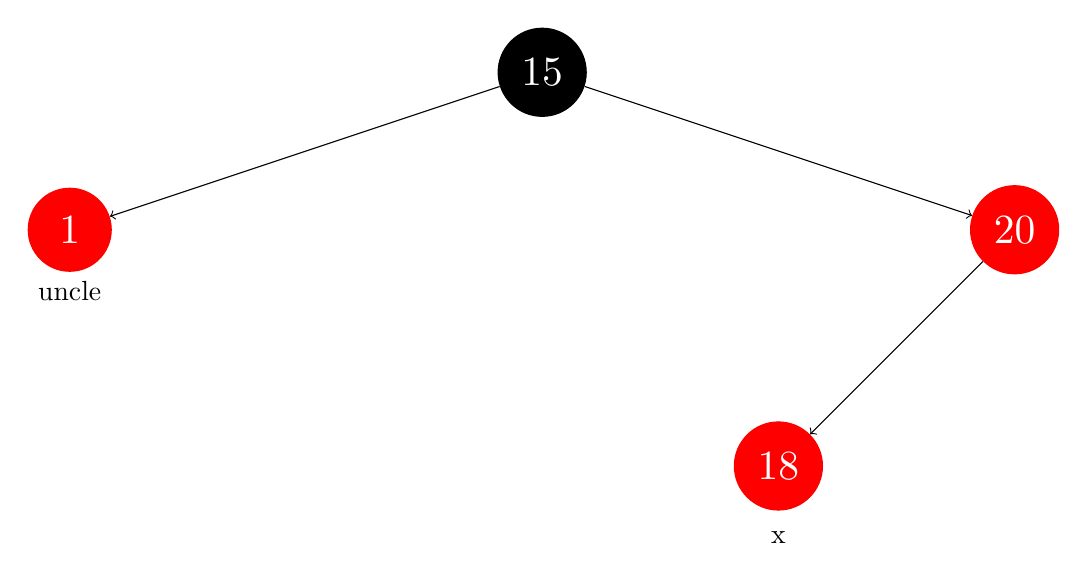
\begin{tikzpicture}
    \node[black] (15) at(10,10) {15};
    \node[red] (1) at(4,8) {1};
    \node[below=15pt] at (4,8) {uncle};
    \node[red] (20) at(16,8) {20};
    \node[red] (18) at(13,5) {18};
    \node[below=20pt] at(13,5) {x};
    \graph{
        (15)->(1);
        (15)->(20)->(18);
    };
\end{tikzpicture}
\\
这颗红黑树违反了红黑树的第4条平衡性质,所以这颗二叉树需要插入调整。
如果红黑树是上文中所绘制的情况,即叔父节点是红色节点,
可以将祖父节点变为红色,父节点变为黑色,这种操作叫做红色上浮。
调整后的红黑树如下图所示:\\
\\
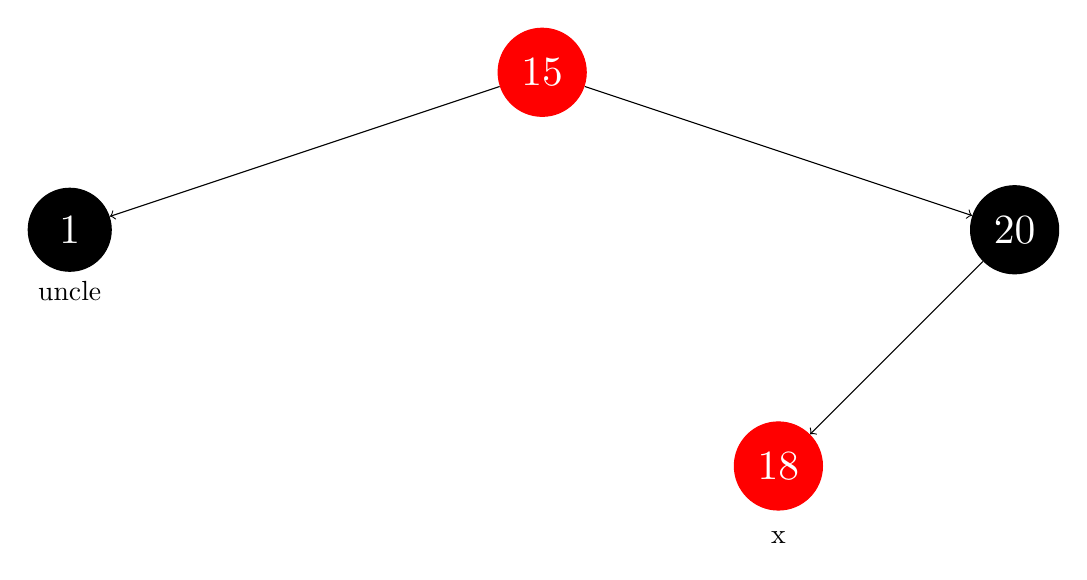
\begin{tikzpicture}
    \node[red] (15) at(10,10) {15};
    \node[black] (1) at(4,8) {1};
    \node[below=15pt] at (4,8) {uncle};
    \node[black] (20) at(16,8) {20};
    \node[red] (18) at(13,5) {18};
    \node[below=20pt] at(13,5) {x};
    \graph{
        (15)->(1);
        (15)->(20)->(18);
    };
\end{tikzpicture}
\\
虽然此时祖父节点为红色,但是祖父节点不一定为整颗红黑树的根节点,
即使是,也可以将根节点手动置为黑色。

第二种情况如下图所示:\\
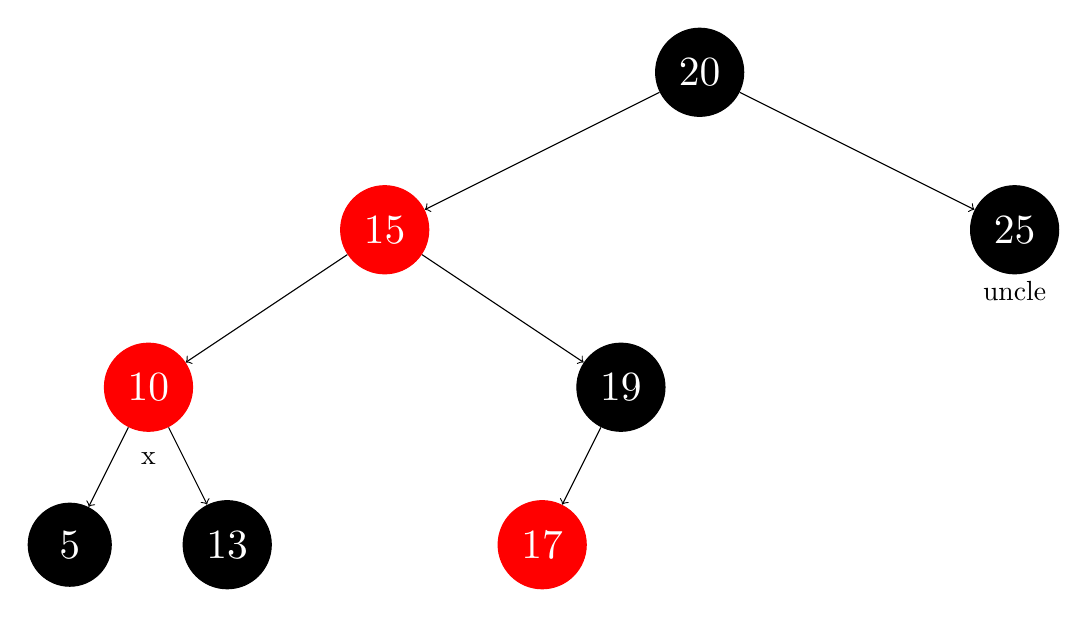
\begin{tikzpicture}
    \node[black,text=white] (20) at(15,10) {20};
    \node[red] (15) at(11,8) {15};
    \node[black] (25) at(19,8) {25};
    \node[red] (10) at(8,6) {10};
    \node[black] (19) at(14,6) {19};
    \node[black] (5) at(7,4) {5};
    \node[black] (13) at(9,4) {13};
    \node[red] (17) at(13,4) {17};
    \node[below=15pt] at(19,8) {uncle};
    \node[below=20pt] at(8,6) {x};
    \graph{
        (20)->(15)->(10)->(5);
        (10)->(13);
        (15)->(19)->(17);
        (20)->(25);
    };
\end{tikzpicture}
\\
在这颗红黑树中,10和15节点是连续的红色节点,违反了
红黑树的第4条平衡性质。所以需要插入调整。

对于这种叔父节点是黑色的情况,像AVL树一样有4种子情况:
祖父节点的左孩子({\color{red}{L}}eft)是红色,
祖父节点的左孩子的左孩子({\color{red}{L}}eft)是红色(LL);
祖父节点的左孩子({\color{red}{L}}eft)是红色,
祖父节点的左孩子的右孩子({\color{red}{R}}ight)是红色(LR);
祖父节点的右孩子({\color{red}{R}}ight)是红色,
祖父节点的右孩子的左孩子({\color{red}{L}}eft)是红色(RL);
祖父节点的右孩子({\color{red}{R}}ight)是红色,
祖父节点的右孩子的右孩子({\color{red}{R}}ight)是红色(RR)。
对于LL类型,可以像AVL树一样,先进行右旋。
右旋之后的红黑树如下图所示:\\
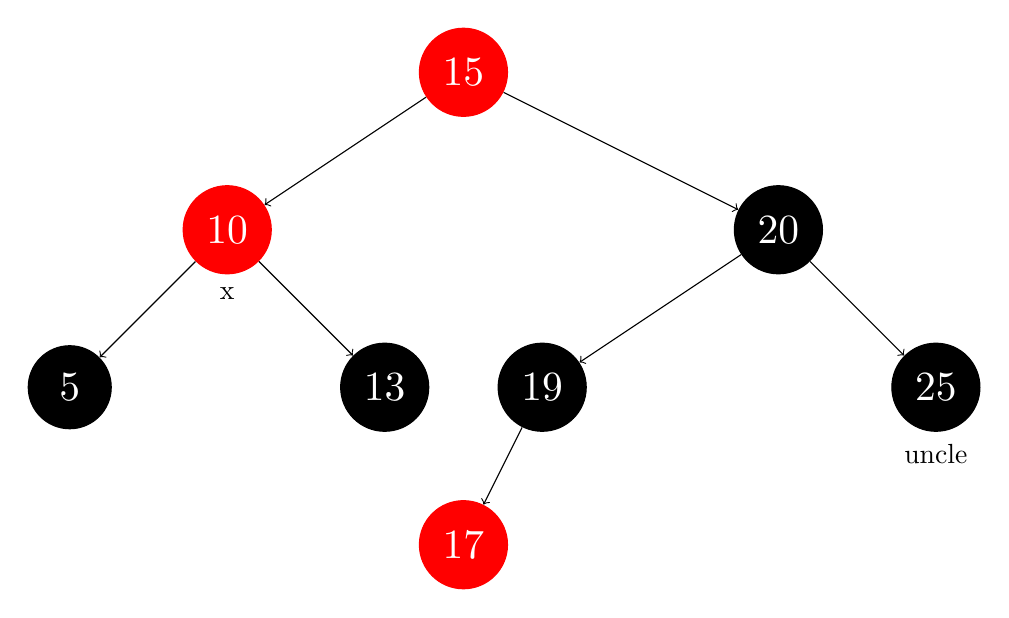
\begin{tikzpicture}
    \node[red] (15) at(10,10) {15};
    \node[red] (10) at(7,8) {10};
    \node[black] (20) at(14,8) {20};
    \node[black] (5) at(5,6) {5};
    \node[black] (13) at(9,6) {13};
    \node[black] (19) at(11,6) {19};
    \node[black] (25) at(16,6) {25};
    \node[red] (17) at(10,4) {17};
    \node[below=1pt of 10] {x};
    \node[below=1pt of 25] {uncle};
    \graph{
        (15)->(10)->(5);
        (10)->(13);
        (15)->(20)->(19)->(17);
        (20)->(25);
    };
\end{tikzpicture}
\\
接下来,请读者思考一个问题:哪些节点的颜色是固定的?
哪些节点的颜色是这颗树的特例\footnote{特例指这个节点的颜色
在其他情况中可能会发生变化}?
解答:\\
首先,根据失衡类型,10、15、25节点的颜色是确定的。
因为15一定是红色,所以20,19一定是黑色。
因为10一定是红色,所以5,13一定是黑色。
综上所述,20、15、25、10、5、13、19的颜色是固定的,
17是特例。

所以,我们只能修改20、15、25、10、5、13、19节点。

为了使每条路线上的黑色节点数量不变,可以将10、20变为黑色,
15变为红色,也就是红色上浮。这样,调整前每条路径上
有2个黑色节点,调整后每条路径上也有2个黑色节点。

调整后的红黑树如下图所示:\\
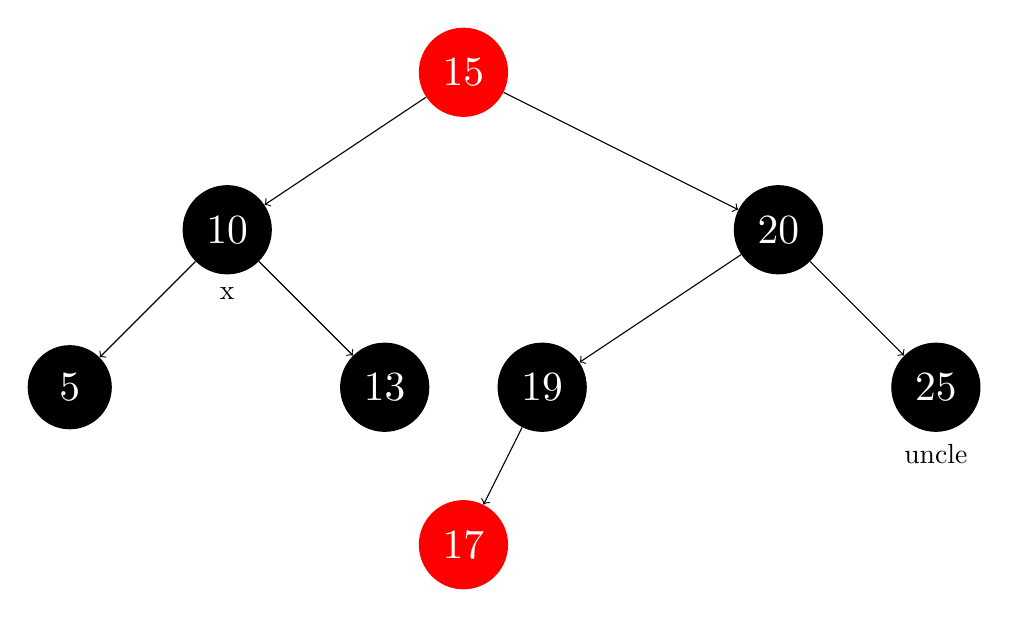
\begin{tikzpicture}
    \node[red] (15) at(10,10) {15};
    \node[black] (10) at(7,8) {10};
    \node[black] (20) at(14,8) {20};
    \node[black] (5) at(5,6) {5};
    \node[black] (13) at(9,6) {13};
    \node[black] (19) at(11,6) {19};
    \node[black] (25) at(16,6) {25};
    \node[red] (17) at(10,4) {17};
    \node[below=1pt of 10] {x};
    \node[below=1pt of 25] {uncle};
    \graph{
        (15)->(10)->(5);
        (10)->(13);
        (15)->(20)->(19)->(17);
        (20)->(25);
    };
\end{tikzpicture}
\\
类似的,LR、RL、RR的方法是先像AVL树一样进行对应的旋转,
再进行红色上浮。

事实上,在最后一步也可以采用红色下沉,即父节点
变为红色,祖父节点变为黑色。

\subsection{删除\texorpdfstring{\cite{delete}}{}}
因为删除度为2的节点可以转化为删除度为1或度为0的节点,所以
下面只讨论删除度为1或度为0的节点的情况。
\begin{table}[H]
    \centering
    \caption{删除方式}
    \label{table:delete}
    \begin{tabular}{|c|c|c|}
        \hline
        \diagbox{\textbf{度}}{\textbf{颜色}} & \textbf{红色} & \textbf{黑色} \\
        \hline
        \textbf{0} & 直接删除 & 生成双重黑节点,触发删除调整 \\
        \hline
        \textbf{1} & 不存在 & 删除节点,唯一子孩子变为黑色,提升唯一子树。 \\
        \hline
    \end{tabular}
\end{table}
不存在度为1的红色节点是因为红色结点的左右孩子都是黑色,如果存在度为1的红色节点,
就会使得某一条路径少一条路径。同理,度为1的黑色节点的唯一子孩子一定是红色,
因为如果度为1的黑色节点的唯一子孩子是黑色,那么就会有一条路径黑色节点少一个。
而删除一个度为0的黑色节点时,某一条路径上的黑色节点就会少一个。这个无处安放的
黑色节点就会加在NIL身上,从而产生双重黑节点。所以,删除调整的目的就是删除双重黑节点。

下面是删除调整的几种情况:
\begin{figure}[H]
    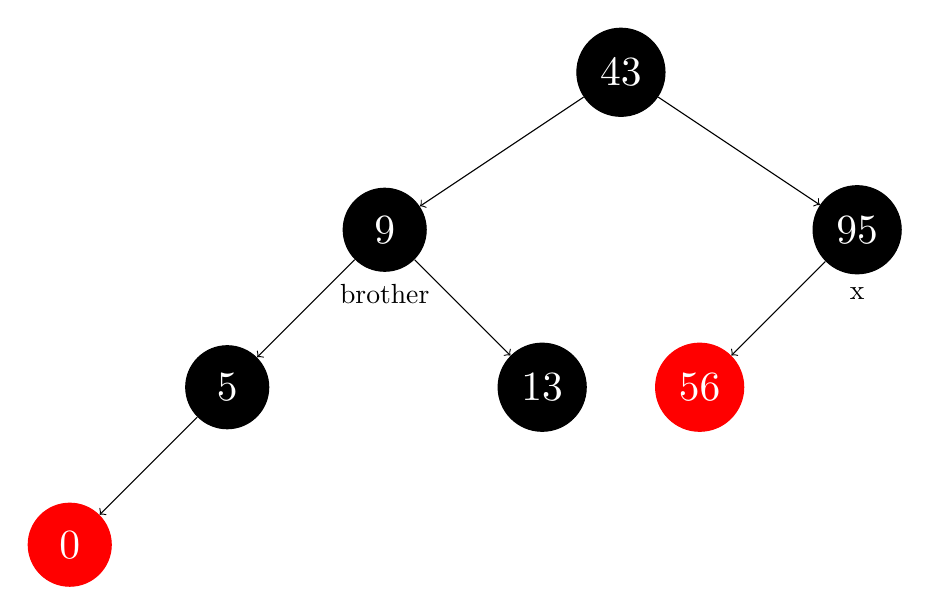
\begin{tikzpicture}
        \node[black] (43) at(10,10) {43};
        \node[black] (9) at(7,8) {9};
        \node[black] (95) at(13,8) {95};
        \node[black] (5) at(5,6) {5};
        \node[black] (13) at(9,6) {13};
        \node[red] (56) at(11,6) {56};
        \node[red] (0) at(3,4) {0};
        \node[below=1pt of 9] {brother};
        \node[below=1pt of 95] {x};
        \graph{
            (43)->(9)->(5)->(0);
            (9)->(13);
            (43)->(95)->(56);
        };
    \end{tikzpicture}
    \caption{删除调整第一种情况}
    \label{fig:delete1}
\end{figure}
如图 \ref{fig:delete1} 所示,若双重黑节点的兄弟节点是黑色,且没有红色子孩子则可以
将父节点颜色加1,即黑变双重黑,红变黑,兄弟节点和双重黑节点颜色减1。

若如下图所示:\\
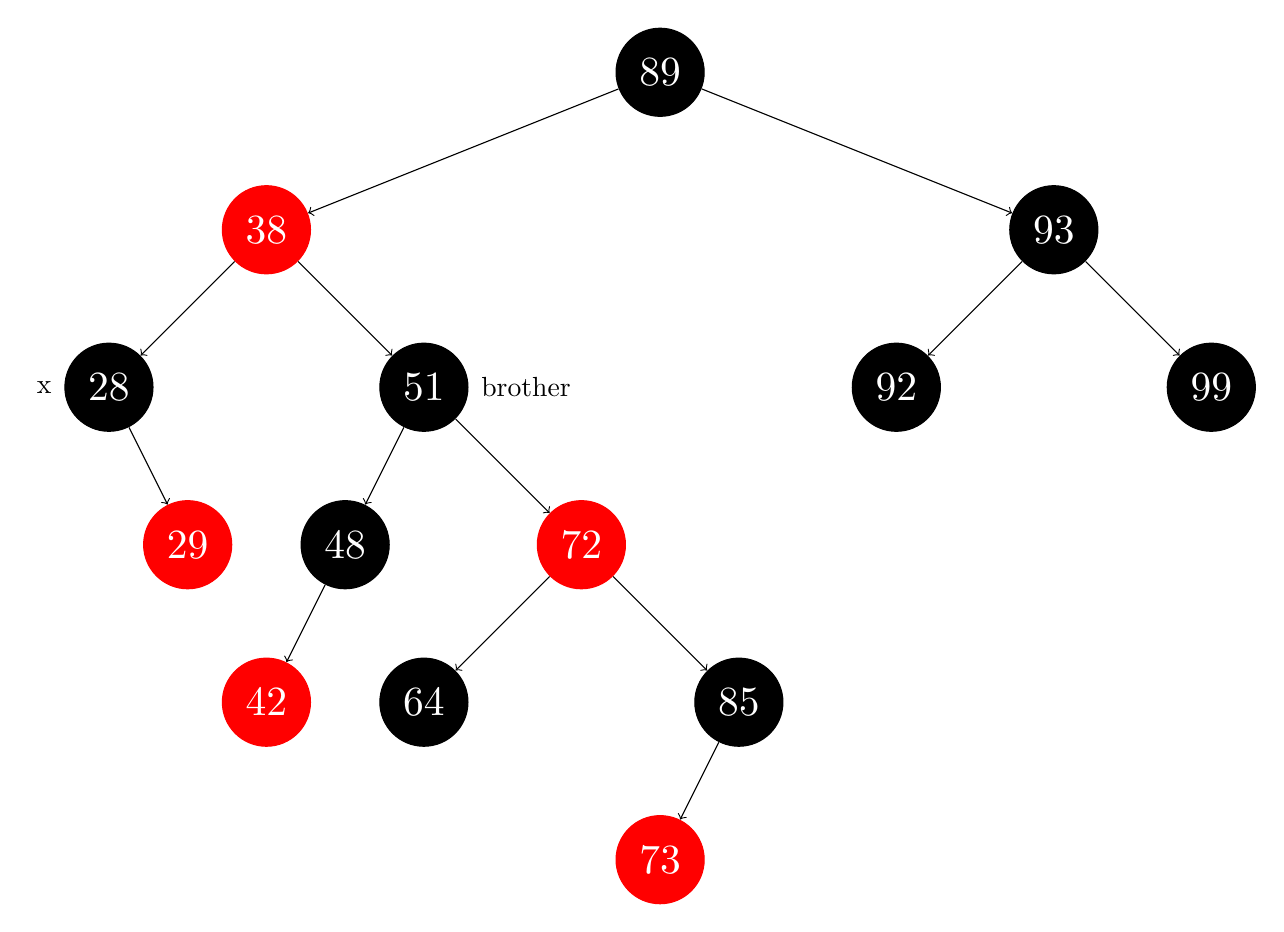
\begin{tikzpicture}
    \node[black] (89) at(10,10) {89};
    \node[red] (38) at(5,8) {38};
    \node[black] (93) at(15,8) {93};
    \node[black] (28) at(3,6) {28};
    \node[black] (51) at(7,6) {51};
    \node[black] (92) at(13,6) {92};
    \node[black] (99) at(17,6) {99};
    \node[red] (29) at(4,4) {29};
    \node[black] (48) at(6,4) {48};
    \node[red] (72) at(9,4) {72};
    \node[red] (42) at(5,2) {42};
    \node[black] (64) at(7,2) {64};
    \node[black] (85) at(11,2) {85};
    \node[red] (73) at(10,0) {73};
    \node[left=1pt of 28] {x};
    \node[right=1pt of 51] {brother};
    \graph{
        (89)->(38)->(28)->(29);
        (38)->(51)->(48)->(42);
        (51)->(72)->(64);
        (72)->(85)->(73);
        (89)->(93)->(92);
        (93)->(99);
    };
\end{tikzpicture}
\\
像这种兄弟节点是黑色,兄弟节点的红色子孩子在兄弟节点相对双重黑节点的同侧上的情况,我们
称之为LL(兄弟节点在双重黑节点的左侧)或RR(兄弟节点在双重黑节点的右侧)。
像这种情况,我们可以像AVL树一样先对38\footnote{删除调整站在父节点处理}进行左旋。左旋完之后如下图所示
\footnote{下图根节点为父节点}:\\
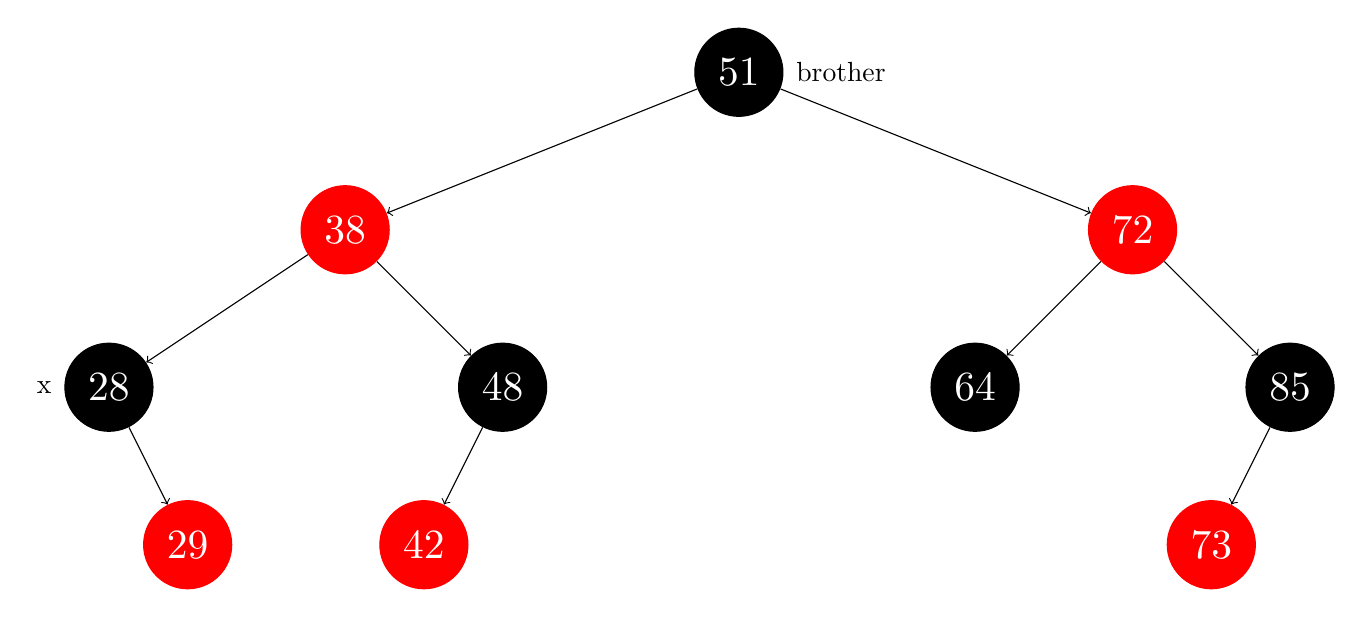
\begin{tikzpicture}
    \node[black] (51) at(10,10) {51};
    \node[red] (38) at(5,8) {38};
    \node[red] (72) at(15,8) {72};
    \node[black] (28) at(2,6) {28};
    \node[black] (48) at(7,6) {48};
    \node[black] (64) at(13,6) {64};
    \node[black] (85) at(17,6) {85};
    \node[red] (29) at(3,4) {29};
    \node[red] (42) at(6,4) {42};
    \node[red] (73) at(16,4) {73};
    \node[left=1pt of 28] {x};
    \node[right=1pt of 51] {brother};
    \graph{
        (51)->(38)->(28)->(29);
        (38)->(48)->(42);
        (51)->(72)->(64);
        (72)->(85)->(73)
    };
\end{tikzpicture}
\\
接下来,请读者思考:哪些节点的颜色是确定的?

可以得到,51、28、72、64、85的颜色是确定的。

因为48可能为红色,所以38应该改为黑色。
修改后发现左侧路径上有3个黑色节点,所以将51变为红色。
51改后又发现,右侧路径上只有1个黑色节点,所以将72变为黑色。

那么,如果38节点原来是黑色呢?在这种情况下,使用这种调整策略
每条路径上的黑色节点会比原来少一个。所以,51应该改成黑色。

综上所述,对于LL和RR类型失衡,应当先进行左旋或右旋,
再将新根节点的颜色修改成原根节点的颜色,最后将新根节点的左右孩子的颜色
修改成黑色。

若如下图所示:\\
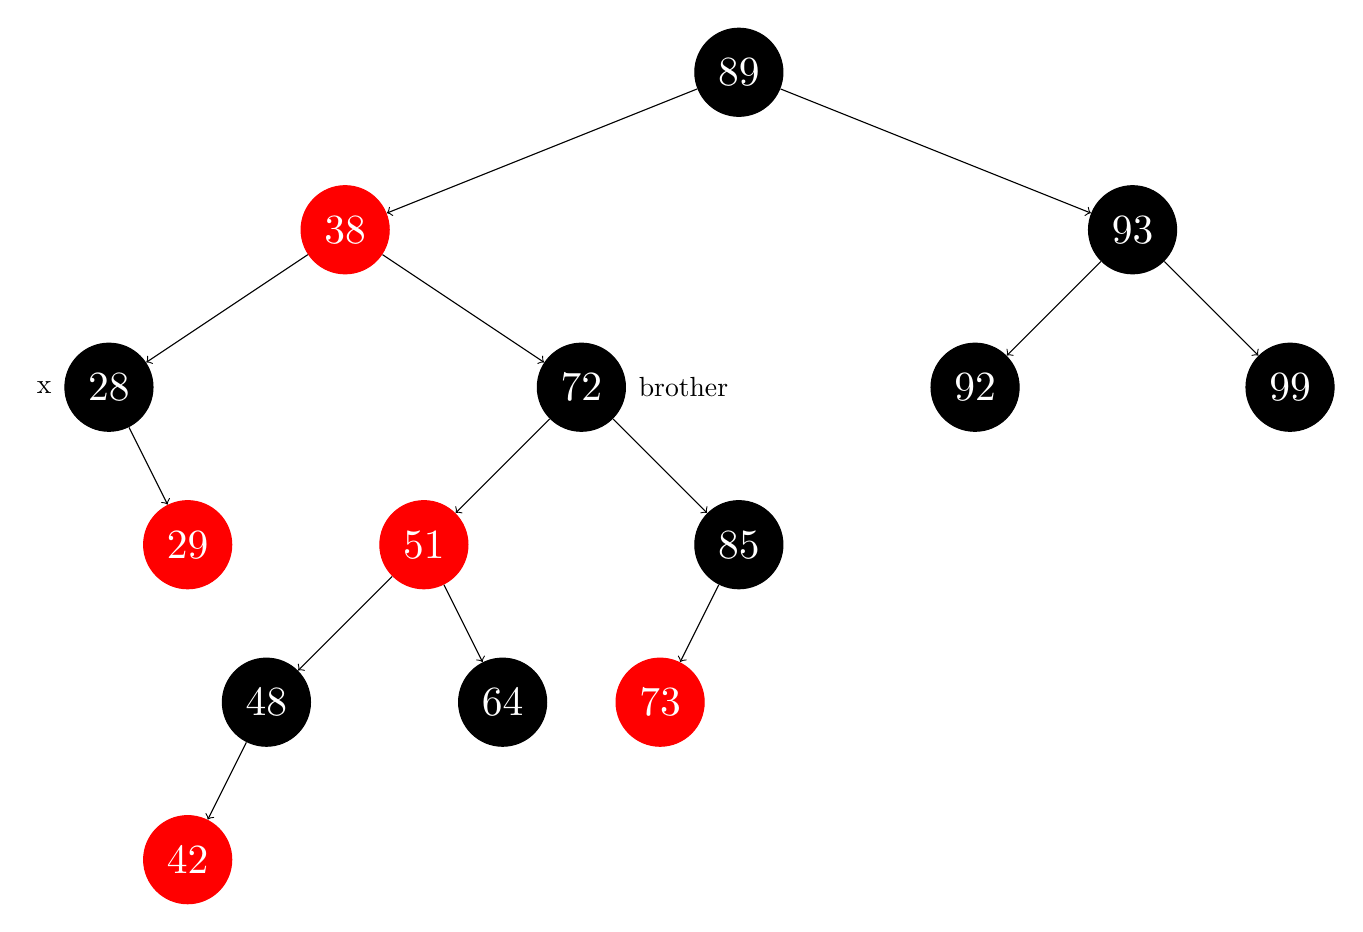
\begin{tikzpicture}
    \node[black] (89) at(10,14) {89};
    \node[red] (38) at(5,12) {38};
    \node[black] (93) at(15,12) {93};
    \node[black] (28) at(2,10) {28};
    \node[black] (72) at(8,10) {72};
    \node[black] (92) at(13,10) {92};
    \node[black] (99) at(17,10) {99};
    \node[red] (29) at(3,8) {29};
    \node[red] (51) at(6,8) {51};
    \node[black] (85) at(10,8) {85};
    \node[black] (48) at(4,6) {48};
    \node[black] (64) at(7,6) {64};
    \node[red] (73) at(9,6) {73};
    \node[red] (42) at(3,4) {42};
    \node[left=1pt of 28] {x};
    \node[right=1pt of 72] {brother};
    \graph{
        (89)->(38)->(28)->(29);
        (38)->(72)->(51)->(48)->(42);
        (51)->(64);
        (72)->(85)->(73);
        (89)->(93)->(92);
        (93)->(99);
    };
\end{tikzpicture}
\\
像这种兄弟节点是黑色,兄弟节点的红色子孩子在兄弟节点相对双重黑节点的异侧上的情况,我们
称之为LR(兄弟节点在双重黑节点的左侧)或RL(兄弟节点在双重黑节点的右侧侧)。
对于这种情况,可以先进行小右旋。右旋之后的红黑树片段如下:\\
\\
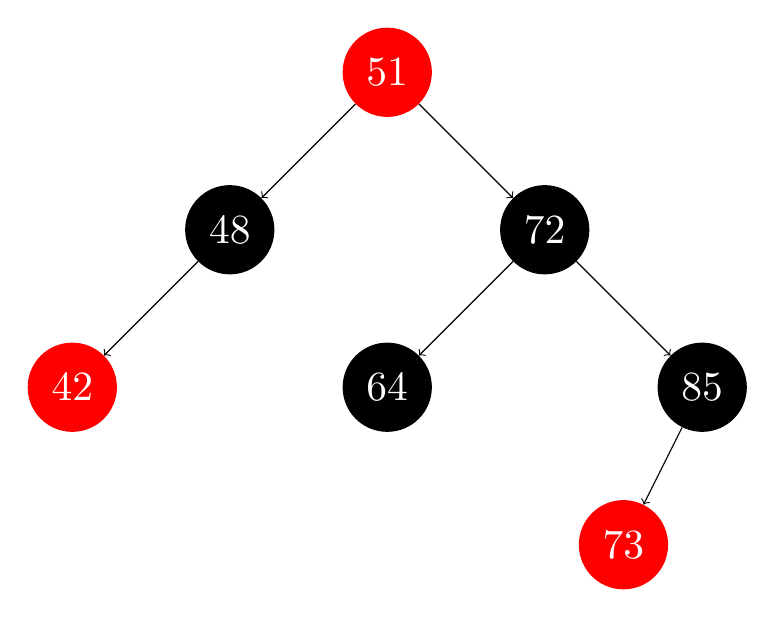
\begin{tikzpicture}
    \node[red] (51) at(10,10) {51};
    \node[black] (48) at(8,8) {48};
    \node[black] (72) at(12,8) {72};
    \node[red] (42) at(6,6) {42};
    \node[black] (64) at(10,6) {64};
    \node[black] (85) at(14,6) {85};
    \node[red] (73) at(13,4) {73};
    \graph{
        (51)->(48)->(42);
        (51)->(72)->(64);
        (72)->(85)->(73);
    };
\end{tikzpicture}

小右旋之后需要调整颜色,但是进行大左旋之后还要调整颜色,所以在代码实现时暂时不调整颜色。

综上所述,先对红黑树进行小右旋或小左旋,转化成LL或RR之后再进行大左旋或大右旋,按LL或RR的方法调整颜色。

若红黑树如下图所示:\\
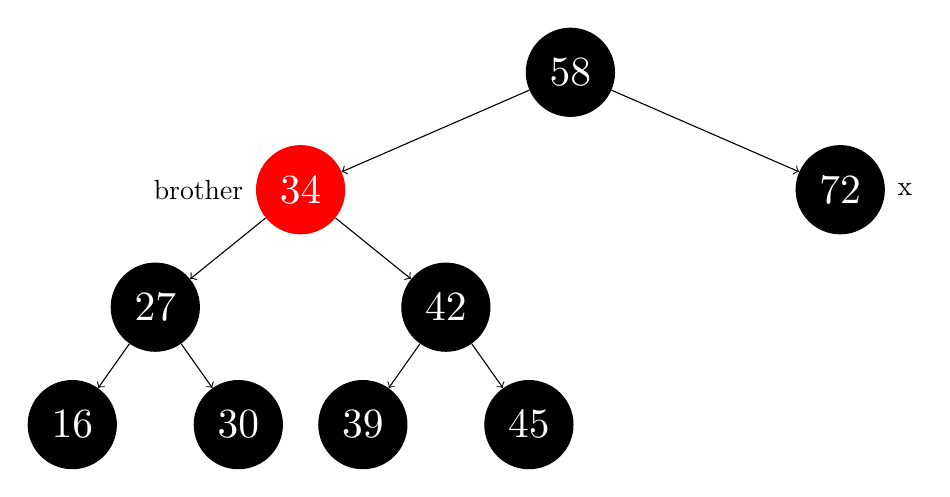
\begin{tikzpicture}
    \node[black] (58) {58};
    \node[red,below=10pt of 58,xshift=-65pt] (34) {34};
    \node[black,below=10pt of 58,xshift=65pt] (72) {72};
    \node[black,below=10pt of 34,xshift=-35pt] (27) {27};
    \node[black,below=10pt of 34,xshift=35pt] (42) {42};
    \node[black,below=10pt of 27,xshift=-20pt] (16) {16};
    \node[black,below=10pt of 27,xshift=20pt] (30) {30};
    \node[black,below=10pt of 42,xshift=-20pt] (39) {39};
    \node[black,below=10pt of 42,xshift=20pt] (45) {45};
    \node[left=1pt of 34] {brother};
    \node[right=1pt of 72] {x};
    \graph{
        (58)->(34)->(27)->(16);
        (27)->(30);
        (34)->(42)->(39);
        (42)->(45);
        (58)->(72);
    };
\end{tikzpicture}
\\
这种情况可以先进行右旋(红色节点在根节点左边)或左旋(红色节点在根节点右边)。右旋之后的红黑树如下图所示:\\
\\
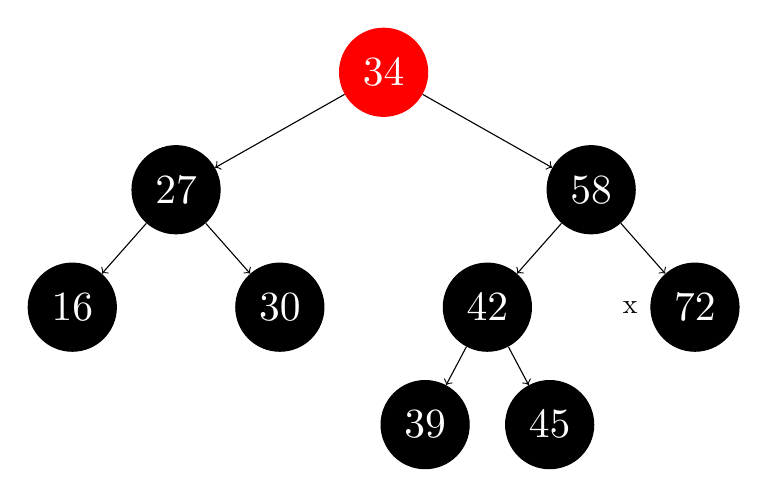
\begin{tikzpicture}
    \node[red] (34) {34};
    \node[black,below=10pt of 34,xshift=-50pt] (27) {27};
    \node[black,below=10pt of 34,xshift=50pt] (58) {58};
    \node[black,below=10pt of 27,xshift=-25pt] (16) {16};
    \node[black,below=10pt of 27,xshift=25pt] (30) {30};
    \node[black,below=10pt of 58,xshift=-25pt] (42) {42};
    \node[black,below=10pt of 58,xshift=25pt] (72) {72};
    \node[black,below=10pt of 42,xshift=-15pt] (39) {39};
    \node[black,below=10pt of 42,xshift=15pt] (45) {45};
    \node[left=1pt of 72] {x};
    \graph{
        (34)->(27)->(16);
        (27)->(30);
        (34)->(58)->(42)->(39);
        (58)->(72);
        (42)->(45);
    };
\end{tikzpicture}
\\
右旋之后,开始调整颜色。

首先,确定哪些节点的颜色是确定的。

可以得出,34、27、58、42、72的颜色是确定的。

因为红黑树左边的路径黑色节点少了一个,所以将34变为黑色。
34改后发现,红黑树右边的路径黑色节点多了一个,所以将58,也就是原根节点改成红色。

修改后红黑树如下:\\
\\
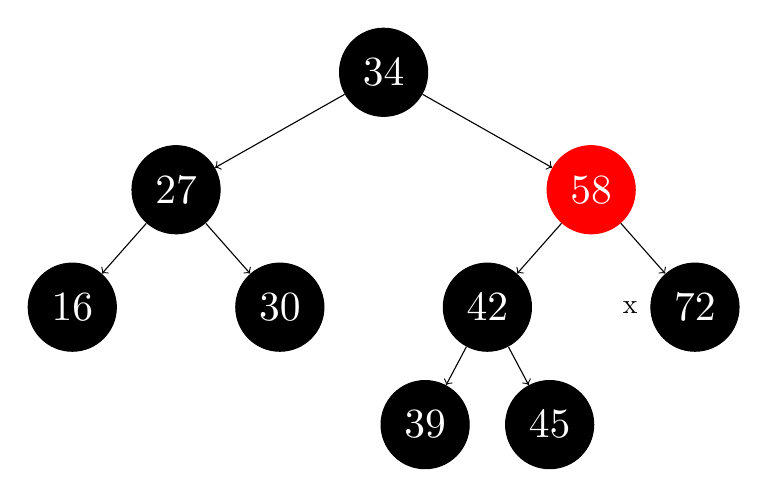
\begin{tikzpicture}
    \node[black] (34) {34};
    \node[black,below=10pt of 34,xshift=-50pt] (27) {27};
    \node[red,below=10pt of 34,xshift=50pt] (58) {58};
    \node[black,below=10pt of 27,xshift=-25pt] (16) {16};
    \node[black,below=10pt of 27,xshift=25pt] (30) {30};
    \node[black,below=10pt of 58,xshift=-25pt] (42) {42};
    \node[black,below=10pt of 58,xshift=25pt] (72) {72};
    \node[black,below=10pt of 42,xshift=-15pt] (39) {39};
    \node[black,below=10pt of 42,xshift=15pt] (45) {45};
    \node[left=1pt of 72] {x};
    \graph{
        (34)->(27)->(16);
        (27)->(30);
        (34)->(58)->(42)->(39);
        (58)->(72);
        (42)->(45);
    };
\end{tikzpicture}
\\

此时,双重黑节点旁边的节点是黑色,可以按前三种情况进行调整。
\newpage
\section{代码演示
    \texorpdfstring{\cite{insert_code}}{}
    \texorpdfstring{\cite{delete_code}}{}}
\begin{framed}
    \lstinputlisting[
        style=C++,
        caption=RedBlackTree.cpp,
        label=RedBlackTree
    ]{../No.8/3.red_black_tree.cpp}
\end{framed}
\bibliographystyle{plain}
\bibliography{quote}
\end{document}